% !TEX root = ./stellar-notes.tex
\section{Shocks}
\newcommand{\gpo}{\ensuremath{(\gamma+1)}}
\newcommand{\gmo}{\ensuremath{(\gamma-1)}}

In a shock, the properties of the fluid change over a scale of a few mean free paths.  Over this distance, the fluid properties---density, pressure, temperature---are not well characterized by smooth, differentiable functions. To understand how shocks arise, imagine a long tube filled with a gas and fitted with a piston at one end. The piston is pushed into the gas; this creates a compressed region of higher density and pressure, and a compression wave propagates into the cylinder.  This behavior can be captured by Burgers's equation,
\[ \frac{\partial u}{\partial t} + \frac{\partial}{\partial x}\left(\frac{u^{2}}{2}\right) = 0, \]
which is simple but has a nonlinear term that captures the formation of a shock.

\begin{figure}
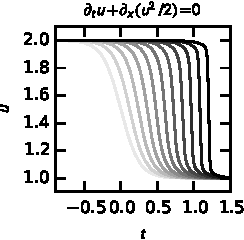
\includegraphics[width=\textwidth]{steepening}
\caption[A disturbance steepening as it propagates.]{The plots show the solution of Burgers's equation for a disturbance propagating along the $x$-direction.  Because the sound speed is greater in the compressed region, the ``back'' of the disturbance $B$ moves faster than the front $F$: as a result, the disturbance steepens.  The disturbance steepens into a shock in a time $t\approx \Delta/(u_{L}-u_{R})$, where $\Delta$ is the initial width of the transition and $u_{L}$ and $u_{R}$ are the values of $u$ on the left and right sides of the disturbance.  }
\label{f.steepening}
\end{figure}

Information about the disturbance is carried by acoustic waves.  In the compressed region, however, the sound speed is higher.  As a result the back of the transition region travels at a faster velocity that the front of the disturbance, so that over time the disturbance steepens (Fig.~\ref{f.steepening}). This steepening continues until the thickness of the transition is small enough that diffusive effects---i.e., viscosity---can balance the steepening.  This gives a characteristic width to the front.  On macroscopic scales, the transition is essentially a discontinuity and is termed a \emph{shock front}.

\begin{marginfigure}
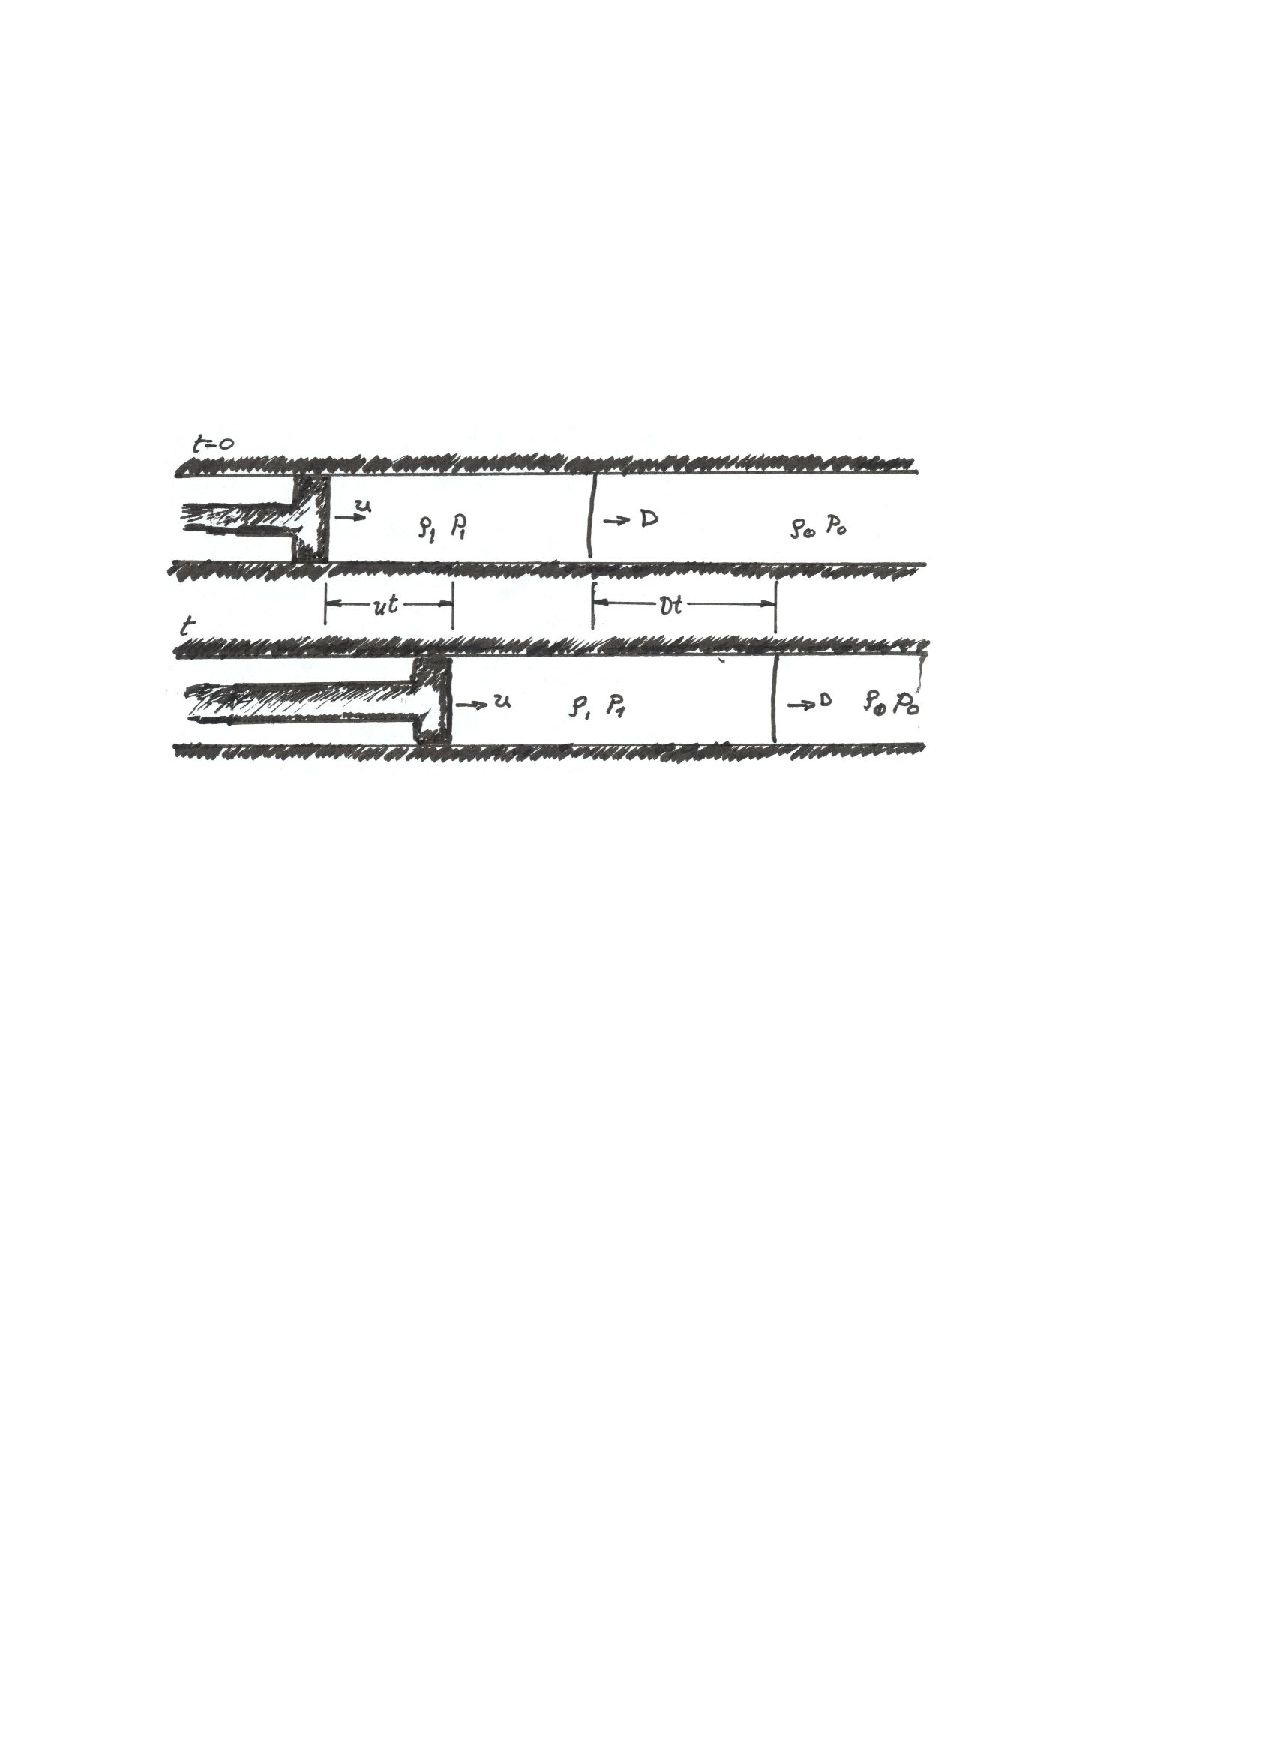
\includegraphics[width=\textwidth]{piston}
\caption[Schematic of a piston driving a shock.]{Schematic of a piston driving a shock.  In this schematic, the shock propagates at velocity $S$.}
\label{f.piston}
\end{marginfigure}

To illustrate the properties of a shock, we'll use our thought experiment of a piston being pushed into a tube filled with gas, as illustrated in Fig.~\ref{f.piston}.  The piston moves to the right with velocity $u$.  We assume that the piston has been pushing the fluid for a while at constant velocity, so that any transients have died down, leaving a simple flow structure at $t=0$ (Fig.~\ref{f.piston}, \emph{top panel}): far from the piston, the fluid is at rest, with density $\rho_{0}$, pressure $P_{0}$, and internal energy $\varepsilon_{0}$; a shock propagates into this fluid with velocity $S$; between the shock and the piston the fluid moves with the same velocity, $u$, as the piston and has density $\rho_{1}$, pressure $P_{1}$, and $\varepsilon_{1}$.

In a time $t$, the piston has moved (Fig.~\ref{f.piston}, \emph{botton panel}) a distance $u\cdot t$, and the shock has moved a distance $S\cdot t$; the mass of the ``shocked'' fluid has therefore increased by $\rho_{1}(S-u)t$.  This must equal the mass swept up by the shock, namely $\rho_{0}St$.  We therefore have our first relation,
\begin{equation}\label{e.shock-mass-1}
\rho_{1}(S-u) = \rho_{0}S.
\end{equation}
The fluid swept up by the shock now has velocity $u$ and thus a momentum $(\rho_{0}St)u$. This increase in momentum must equal the net impulse imparted to the fluid, $(P_{1}-P_{0})t$.  We therefore have our second relation,
\begin{equation}\label{e.shock-momentum-1}
S_{1} - S_{0} = S\rho_{0}u.
\end{equation}
The fluid swept up by the shock has a change in total energy, $(\rho_{0}S t)(\varepsilon_{1} + u^{2}/2 -\varepsilon_{0})$. This must equal the work done on the fluid by the piston, which is the force times displacement $P_{1}ut$.  We therefore have our third relation,
\begin{equation}\label{e.shock-energy-1}
\rho_{0}S\left[\varepsilon_{1}-\varepsilon_{0} + \frac{1}{2}u^{2}\right] = P_{1}u.
\end{equation}
To abstract the problem, we transform to a frame moving with the shock.  In this frame the upstream velocity ahead of the shock has velocity $u_{0} = -S$; the downstream velocity is $u_{1} = u-S$.  The difference in velocity is $|u_{0} - u_{1}| = u$.
In this frame, equations~(\ref{e.shock-mass-1}), (\ref{e.shock-momentum-1}), and (\ref{e.shock-energy-1}) take on the more familiar forms,
\begin{eqnarray}
\rho_{1}u_{1} &=& \rho_{0}u_{0},\label{e.shock-mass-2}\\
P_{1} + \rho_{1}u_{1}^{2} &=& P_{0} + \rho_{0}u_{0}^{2},\label{e.shock-momentum-2}\\
(\rho_{1}u_{1})\left[\varepsilon_{1} + \frac{1}{2}u_{1}^{2} + \frac{P_{1}}{\rho_{1}}\right] &=& 
	(\rho_{0}u_{0})\left[\varepsilon_{0} + \frac{1}{2}u_{0}^{2} + \frac{P_{0}}{\rho_{0}}\right]. 
			\label{e.shock-energy-2}
\end{eqnarray}
Recognize these?  Compare with equations~(\ref{e.mass-1}), (\ref{e.momentum-2}), and (\ref{e.energy-2}), and recognize that equations~(\ref{e.shock-mass-2}), (\ref{e.shock-momentum-2}), (\ref{e.shock-energy-2}) just express that the downstream mass flux, momentum flux, and energy flux equal their upstream counterparts.

Equations~(\ref{e.shock-mass-2}), (\ref{e.shock-momentum-2}), (\ref{e.shock-energy-2}), when supplemented with an equation of state, are sufficient to allow solution for $P_{1}$ and $\rho_{1}$ in terms of $P_{0}$, $\rho_{0}$ and $u$. To explore the properties of the shock, we adopt a simple ideal adiabatic equation of state: $P =  (\gamma - 1)\rho\varepsilon = K \rho^{\gamma}$ with sound speed $c^{2} = \gamma P/\rho$.  The enthalpy is then
\[ \varepsilon + \frac{P}{\rho} = \frac{\gamma}{\gamma-1}\frac{P}{\rho}. \]
Using this equation of state, we can reduce equations~(\ref{e.shock-mass-2}), (\ref{e.shock-momentum-2}), (\ref{e.shock-energy-2}) into expressions in terms of the pressure ratio $P = P_{1}/P_{0}$:
\begin{eqnarray}
	\textrm{density ratio,}&\qquad& \frac{\rho_{1}}{\rho_{0}} 
			= \frac{\gpo P + \gmo}{\gmo P +  \gpo};\\
	\textrm{entropy increase,} &\qquad& s_{1}-s_{0} 
		= c_{v}\ln\left[\frac{P_{1}}{P_{0}}\left(\frac{\rho_{0}}{\rho_{1}}\right)^{\gamma}\right];\\
	\textrm{temperature ratio,} &\qquad& \frac{T_{1}}{T_{0}} = \frac{P_{1}}{P_{0}}\frac{\rho_{0}}{\rho_{1}};\\
	\textrm{upstream Mach,} &\qquad& \left(\frac{u_{0}}{c_{0}}\right)^{2} = \frac{\gpo P + \gmo}{2\gamma};\\
	\textrm{downstream Mach,} &\qquad& \left(\frac{u_{1}}{c_{1}}\right)^{2} 
			= \frac{\gmo P + \gpo}{2\gamma P}.
\end{eqnarray}
In the limiting case of a strong shock, $P \gg 1$, the density increase is finite: $\rho_{1}/\rho_{0} \to \gpo/\gmo$; for $\gamma = 5/3$, $\rho_{1}/\rho_{0}\to 4$.  The temperature and entropy jumps across the shock, however, scale with $P$ and are arbitrarily large.  The upstream Mach number is likewise proportional to the pressure ratio, $\Ma_{0}^{2} \to \gpo P/(2\gamma)$, but the downstream flow is subsonic, $\Ma_{1}^{2} \to \gmo/(2\gamma)$. The shock transforms the ordered (low-entropy) supersonic upstream flow into the disordered (high-entropy) subsonic downstream flow.
